\documentclass[12pt]{article}
\usepackage{amsmat}
\usepackage[margin = 1in]{geometry}
\usepackage{graphicx}
\usepackage{booktabs}
\usepackage{natbib}
\usepackage{lipsum}
\usepackage[colorlinks=true, citecolor=blue]{hyperref}



\title{Baseball Team Hitters Dicipline Stats}
\author{Chenyu Mu\\
  Department of Statistics\\
  University of Connecticut
}

\begin{document}
\maketitle

\begin{abstract}
    Accuracy data and appropriate method of measure is a crucial step towards building a successful career performance for Baseball players. 
This paper provides valuable insights and performace data on 2023 Baseball Team.
\end{abstract}
\end{abstract}


\section{Introduction}
\label{sec:intro}
Baseball Hitters' performance is critical for a team in competetions. 
However, only based on several competitions, we cannot get accuracy perfomance results. 
Thus, we should use appropriate method to calculate and observe the trend of hitters' performance. 
I use the 2022 and 2023 data to show the right way to calculate the perfromance and conclude the data results. 


\lipsum[1-2]

To cite a reference, here are examples.

The data is from UConn baseball website \citet{BSB2023seasonStats}  \lipsum[1]
The definition of baseball terms.\citet{Platedicipline}. \lipsum[2]


% roadmap
The rest of the paper is organized as follows.
The data will be presented in Section~\ref{sec:data}.
The methods are described in Section~\ref{sec:meth}.
The results are reported in Section~\ref{sec:resu}.
A discussion concludes in Section~\ref{sec:disc}.


\section{Data}
\label{sec:data}

The data is from UConn baseball 2023. Following are definitions we may use:
**AB** at bats 
**AVG**batting average 
**BB**bases on balls 
**ER**earned runs
**H**hits; holds
**K**killed 
**OBP**on base percentage

\begin{equation}
  \label{eq:avg}
  AVG= H/AB
\end{equation}
which states that the average hit number of hitters.
\lipsum{1}

\section{Methods}
\label{sec:meth}
$O-Contact$ is the amount of contact a batter makes on pitches outside of the zone, 
which is generally a bad thing. 
$Z-Contact$ is the amount of contact on pitches in the strike zone, which is a very good thing. 
These are the pitches you can drive, and if you are missing on a lot of pitches in the zone (which should be the easiest pitches to hit), 
you are going to strug   gle to hit for average.

\begin{equation}
  \label{eq:Contact}
  \Contact = 100*(Swing-Missing)/swing.
\end{equation}

Equation~\eqref{eq:Contact} is interesting. \lipsum[1-4]



\section{Results}
\label{sec:resu}

Table~\ref{tab:rv} The table show the Players' average percentage and the number of at batting and hit pitches number.
\lipsum[1-4]

\begin{table}[tbp]
  \caption{Here is the first table}
  \label{tab:rv}
\centering
\begin{tabular}{rrr}
 \toprule
 Player & AVG & AB & H \\ 
 \midrule
 Broadhurst Luke & 0.312 & 205 & 64\\
 Morton Korey & 0.290 & 224 & 65\\
 Daniels Ryan & 0.273 & 110 & 30\\
 Hyde Ryan & 0.250 & 60 & 15\\
 \bottomrule
\end{tabular}
\end{table}

Figure~\ref{fig:stat} shows the distance against the speed from this dataset.


\begin{figure}[tbp]
  \centering
  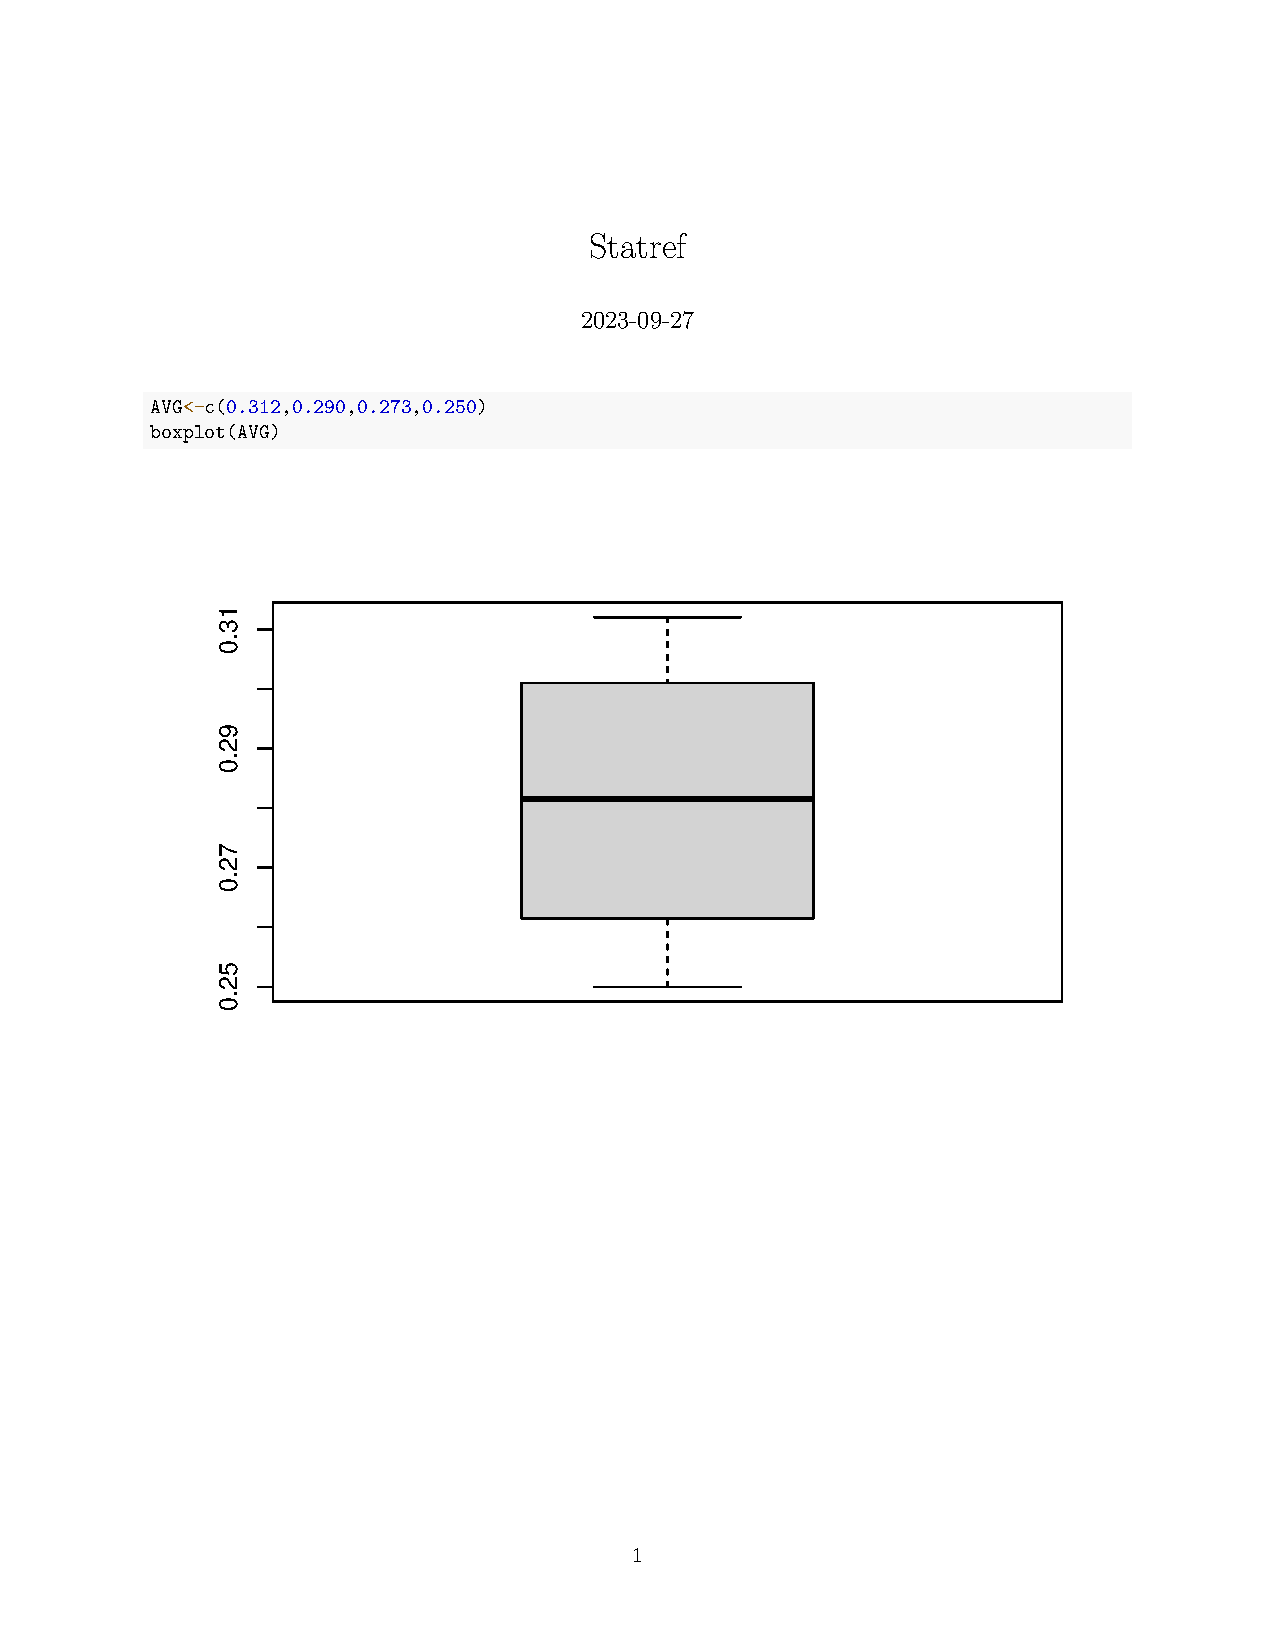
\includegraphics[width=\textwidth]{stat.pdf}
  \caption{This is players' AVG boxplot.}
  \label{fig:stat}
\end{figure}

\section{Discussion}
\label{sec:disc}

This provides the insight of players' performance trend, I can use the result to decide the future training content.

\lipsum[1-2]
Watch for prevalence of diabetes \citep{wild2004global}.

\bibliography{refs}
\bibliographystyle{mcap}

\end{document}